\subsection{Predicting the size of a core composition}
In Section~\ref{sec:streamit:dse}, Figure~\ref{fig:threadtrend} showed the performance of each of the 15 benchmarks when partitioning them into threads with and without core-composition.
In both cases, the number of threads is often similar.
The section also demonstrated that loop unrolling can improve the performance of core composition.

Since core composition is used to improve the performance of a single-working-thread, it is important to take into consideration that partitioning the software into threads facilitates the core estimation per thread.
Without determining a number of threads before predicting the number of cores the core-composition model has no information as to the number of threads or the structure of each thread.
In this situation, the core-composition model would either have to make its own estimates as to the thread count, or make a general prediction for a single-working-thread.
Therefore predicting core-composition comes after predicting the number of threads.

\subsubsection{Gathering Training Data for Core-Composition}
For this section the single-working-threaded version of the StreamIt benchmark are used to determine the optimal number of cores in order to explore all possible core composition sizes.
Some of the multi-threaded versions of benchmarks can be used to add extra data-points to build the model, however not all thread-counts are suitable.
One of the difficulties of adding data-points from the highly threaded versions of an applications is that each thread will only be able to have a very small core-composition.
For example, if the 15 threaded version of a benchmarks is added as data points to the model, then each of the feature vectors for this version would have a single core attributed to it.
This is due to the fact that in the 15 threaded versions of benchmarks each thread can only have a single core due to the number of cores on the DMP.
Yet, these threads could potentially benefit from core-composition, so adding them as data points to the model skews future predictions as the feature vector for each thread would associate the features to use only a single core.
Thus high-threaded versions of applications must be ignored to avoid having incorrect suggestions for core-composition sizes.

For the exploration of core composition, the 15 StreamIt benchmarks explored throughout the design space exploration are used. %explain why.
To increase the amount of data available, multiple versions of the benchmarks using different amounts of unrolling are included in the search space.
Four different levels of unrolling are used in to build the model: 0,4,16 and 64.
To determine the optimal number of cores only the training data that has a performance within 1\% of the best is selected.

\begin{figure}[t]
\centering
  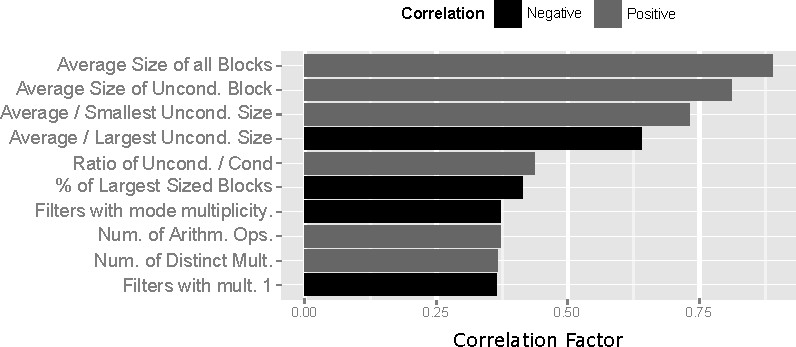
\includegraphics[width=1\textwidth]{streamit-paper/graphics/corrGraph_remix2.pdf}
  \caption{The ten highest correlating features with the optimal number of cores.}\label{fig:corrCore}
\end{figure}


\subsubsection{Correlation Analysis}

Figure~\ref{fig:corrCore} shows the highest correlating features with the optimal number of cores.

The ten features can be described as follows
\begin{itemize}
\item Average Size of All Blocks: Average number of operations per block of code.
\vspace{-1em}
\item Average Size of Unconditional Blocks: Average number of operations per blocks that must execute unconditionally.
\vspace{-1em}
\item Average / Smallest Unconditional Size: The ratio between the average size of a block compared to the smallest size of unconditional blocks.
\vspace{-1em}
\item Average / Largest Unconditional Size: The ratio between the average size of a block compared to the largest size of unconditional blocks.
\vspace{-1em}
\item Ratio of Unconditional Blocks to Conditional Blocks.
\vspace{-1em}
\item Percentage of blocks that have the largest number of operations.
\vspace{-1em}
\item Filters with mode multiplicity: number of filters that have the average mode multiplicity.
\vspace{-1em}
\item Number of arithmetic operations found in the program.
\vspace{-1em}
\item Number of distinct multiplicites found in the program.
\vspace{-1em}
\item Number of filters that have a multiplicity of 1.
\end{itemize}


The features are very different from the ones presented in Figure~\ref{fig:corr} and overall there are features which correlate higher with core-compositions than number of threads.
The highest correlating value, which is the average size of a block, has a correlation factor of 0.88.
It is important to note that the concept of an operation here is at the StreamIt level and not the architectural level.
This is because the machine learning model will get information from the source-level StreamIt translation.
With that in mind, the number of operations will correlate with number of instructions found at the instruction level.

The second feature is similar to the first but only takes into account blocks that will be executed unconditionally.
Blocks found in loops are excluded for this metric as there is still some form of condition for those blocks to be executed, they are counted as conditional.
The next two feature compare the size of the average size of an unconditional block to the largest and smallest unconditional block.
The fifth feature measures the ratio of the number of unconditional blocks to conditional.

Overall the highest correlating features are not features distinct to StreamIt, such as Pipelines or SplitJoins.
This is due to the fact that, from a single-threaded perspective, SplitJoins and Pipelines are less visible in terms of performance.
This is especially true of SplitJoins as they will not be distributing data amongst different threads and, technically, a single-threaded StreamIt program is a long pipeline structure.
It can thus be inferred that the optimal number of cores is independent of the structure of a StreamIt program.
Instead determining the correct core-composition is more dependent on the amount of computation found in each program.

From Figure~\ref{fig:corrCore} the highest correlating features fit naturally under the assumptions that higher core compositions will perform better with larger blocks of operations and thus blocks of instructions.
When blocks are small, a single core can fetch and execute multiple blocks in parallel; up to 4 blocks per core when blocks are smaller than 32 instructions.
Cores in a composition do not fetch blocks independently; instead one of the cores in the composition will start by fetching blocks until it all its lanes are used and then submits the following predicted PC to the next core in the composition.
If blocks are small this means that core-compositions will have to predict a high amount of blocks to fill up all its cores.
Thus large blocks reduce the amount of predictions required to populate all the cores with blocks, reducing the latency of fetching blocks for all cores.
The necessity to correctly predict blocks to ensure that all cores are fully utilised explains why a higher number of unconditionally executed blocks compared to conditional blocks correlates positively with large core compositions.

The importance of size is also apparent as the difference between the largest block size and the average block size negatively correlates with core-composition.
The ratio of unconditional and conditional blocks is considered less important than block size due to branch prediction, however having a larger number of unconditional branches is a natural fit for larger core-compositions as it reduces the dependency on high branch-prediction accuracy.

Other features that are analysed included more fine-grained data such as the types of operations that are found in the blocks of code.
This involved finding ratios of floating point, integer and memory operations.
However, according to the correlation graph in Figure~\ref{fig:corrCore}, the constitution of these blocks of code is not as important as their size or whether they are conditionally executed.

\begin{figure}[t]
  \center
  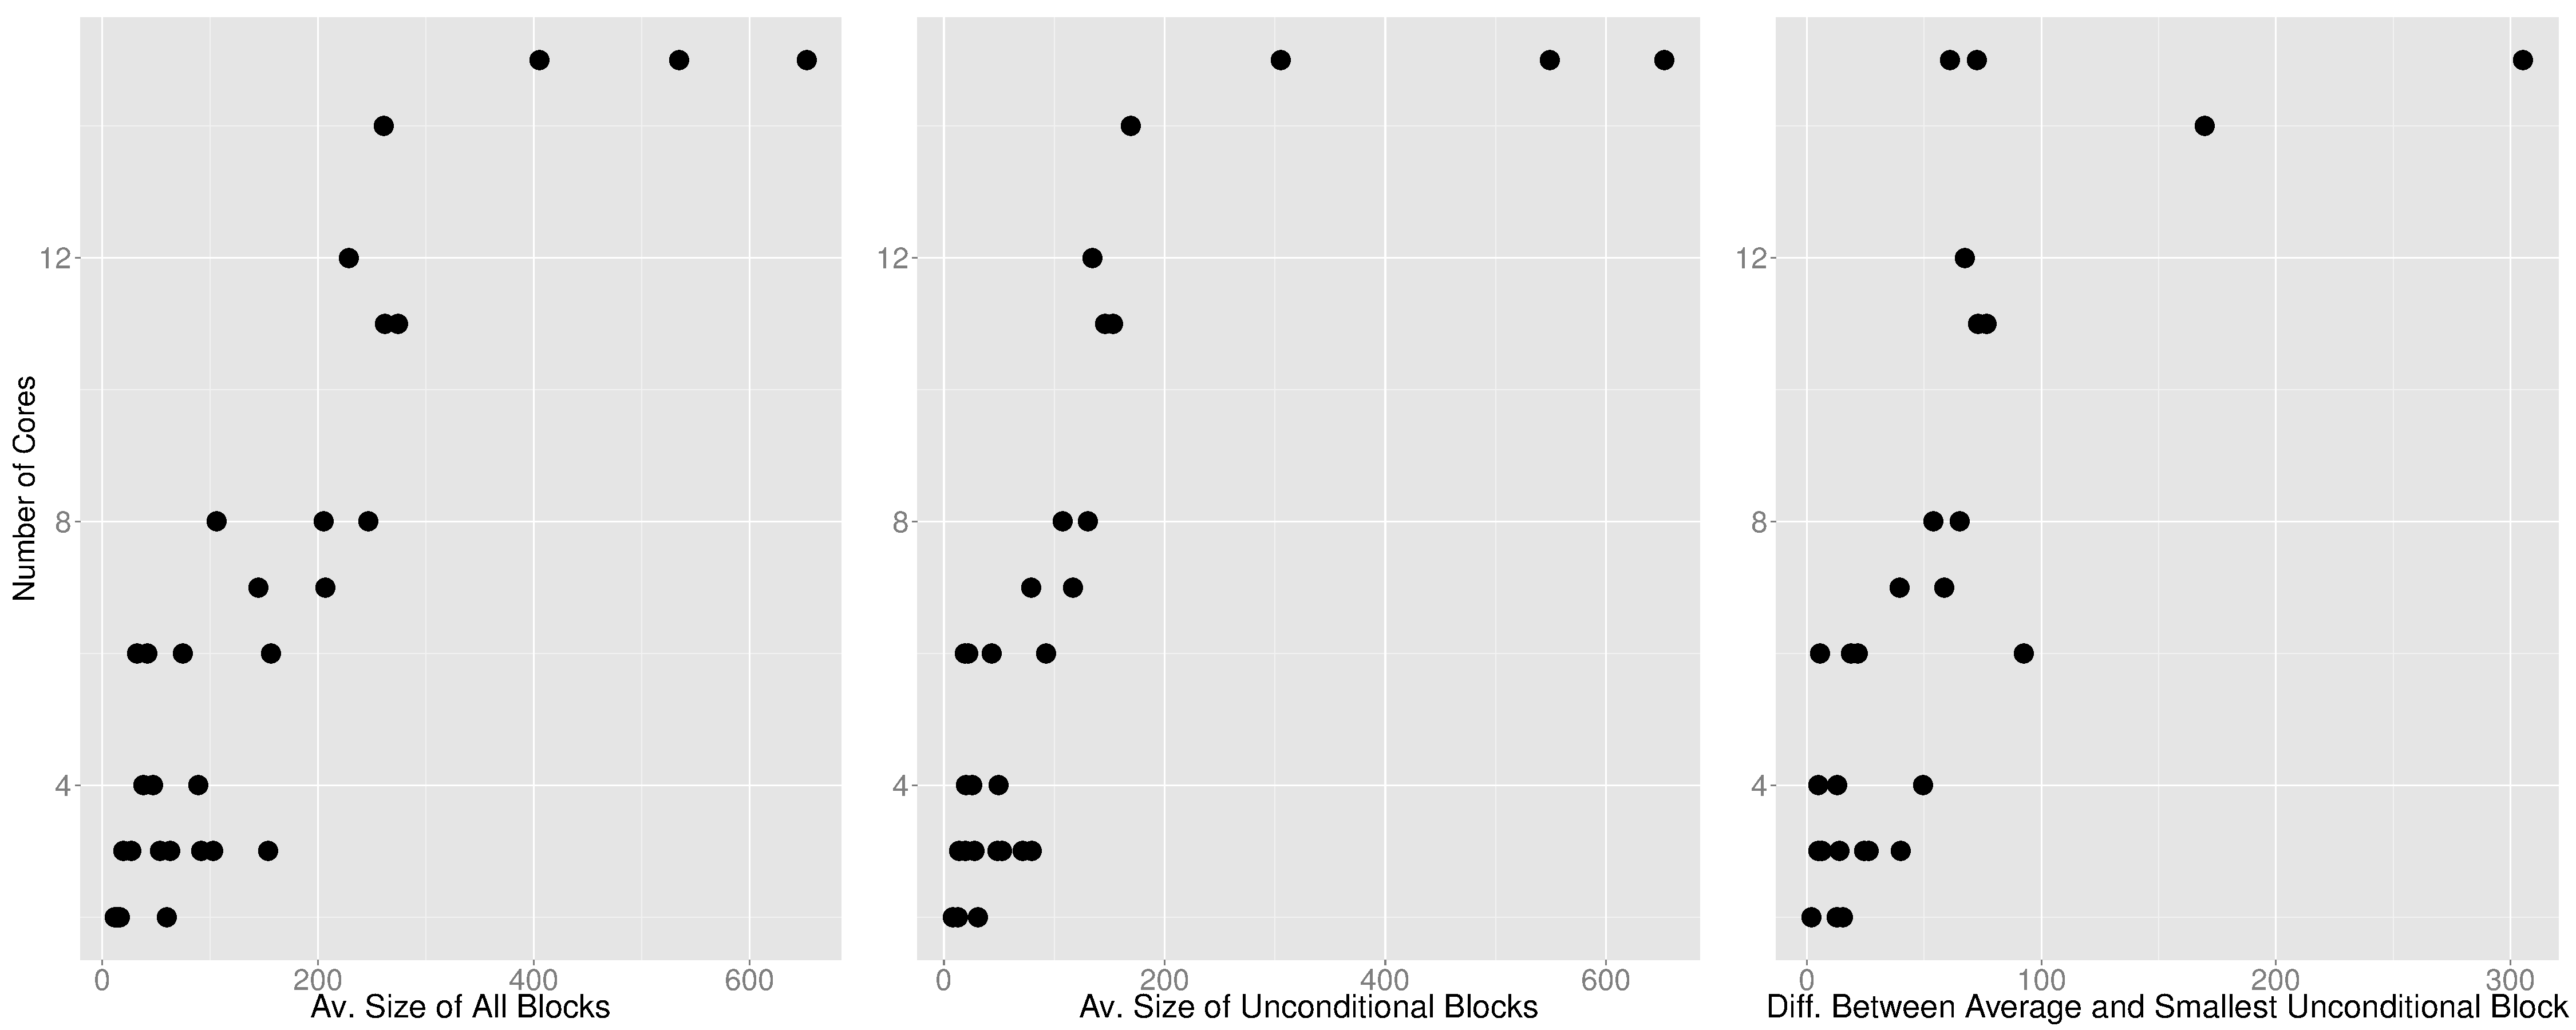
\includegraphics[width=1\textwidth]{streamit-paper/graphics/lineargraphs.pdf}
  \caption{Optimal number of cores in relation to the three highest correlating features. The maximum number of cores plateaus on the right hand side as this is the maximum possible amount.}\label{fig:maxav}
\end{figure}

\subsubsection{Linear Regression Model}
Given that the optimal number of cores highly correlates with a few features, a linear regression is a natural choice to predict the best number of threads.
Figures~\ref{fig:maxav} represent how the first three highest correlating values affect the optimal number of cores for a single-working-thread.
This figure is obtained by finding the best number of cores for the single-working-threaded version of each of the StreamIt benchmarks whilst varying the amount of loop unrolling.
It is important to note that the reason the points in the top right corner appear to converge at 15 cores is due to the fact that no more than 15 cores can be fused.
Overall, Figure~\ref{fig:maxav} shows that StreamIt applications with large unconditionally executed blocks will require large compositions.


